\section{Workload Characterization}
\label{sec:workloadchar}



Comparing the trends observed in Spider I vs Spider II



\subsection{I/O Usage Trends}

\subsubsection{Read vs Write}

%\subsubsection{Atlas1 and Atlas2 Utilization}

Figure~\ref{fig:rwratio} shows the read vs. write balance observed on the
Spider 2 system.  As can be seen, there is a slight imbalance in the total
write requests for 50\% of the controllers sampled. This imbalance is because
the upper level file systems are imbalanced. As we stated above we deployed to
file system namespaces on  non-overlapping hardware resources. The file systems
are allocated across projects at the OLCF and some projects have been heavier
I/O consumers than others; it turns out that the ``atlas1'' partition is being
utilized at a higher rate.  In general we see a higher percentage of write
operations on Spider 2 as compared to Spider 1. This meets our design
expectations for handling large memory checkpoints with a minimal reading of
those checkpoint data files.


Figure~\ref{fig:rwratio} shows the read and write ratios on Spider 1 and 2
storage systems. As can be seen, on Spider 1 60\% of the I/O workload was write
operations and 40\% was reads. Spider 1 was a center-wide shared resource
across all OLCF platforms, and high percent of the read requests was attributed
to analysis and data transfer I/O workloads accessing Spider 1. 

Spider 2 is also a center-wide shared resource, and a similar trend can be
observed. However, the percent of reads on Spider 2 is less compared to Spider
1, and they amount to roughly 25\%. This can be attributed to large-data
transfers into Spider 2 from various resources currently going on for later
processing on Titan. Also it is quite visible in Figure~\ref{fig:rwratio}(b)
that Atlas1 portion of the Spider 2 is 10\% more write-intensive than the
Atlas2 (left half vs. right half of the Figure~\ref{fig:rwratio}(b). This
discrepancy is due to a user project allocation problem we encountered early
on. User projects were categorized in terms of science domains and expected I/O
requirements equally on Atlas1 and Atlas2 portions when Spider 2 was turned
into production. However, our expectation did not materialize completely, and
since then we have been observing more I/O on Atlas1 compared to Atlas2. We
have taken steps (e.g. moving some user projects from Atlas1 to Atlas2) to
rectify this mismatch and over the time it is expected that both portions will
be exercised with roughly equivalent I/O workloads. 

\begin{figure}[!t]
\begin{center}
\begin{tabular}{c}
{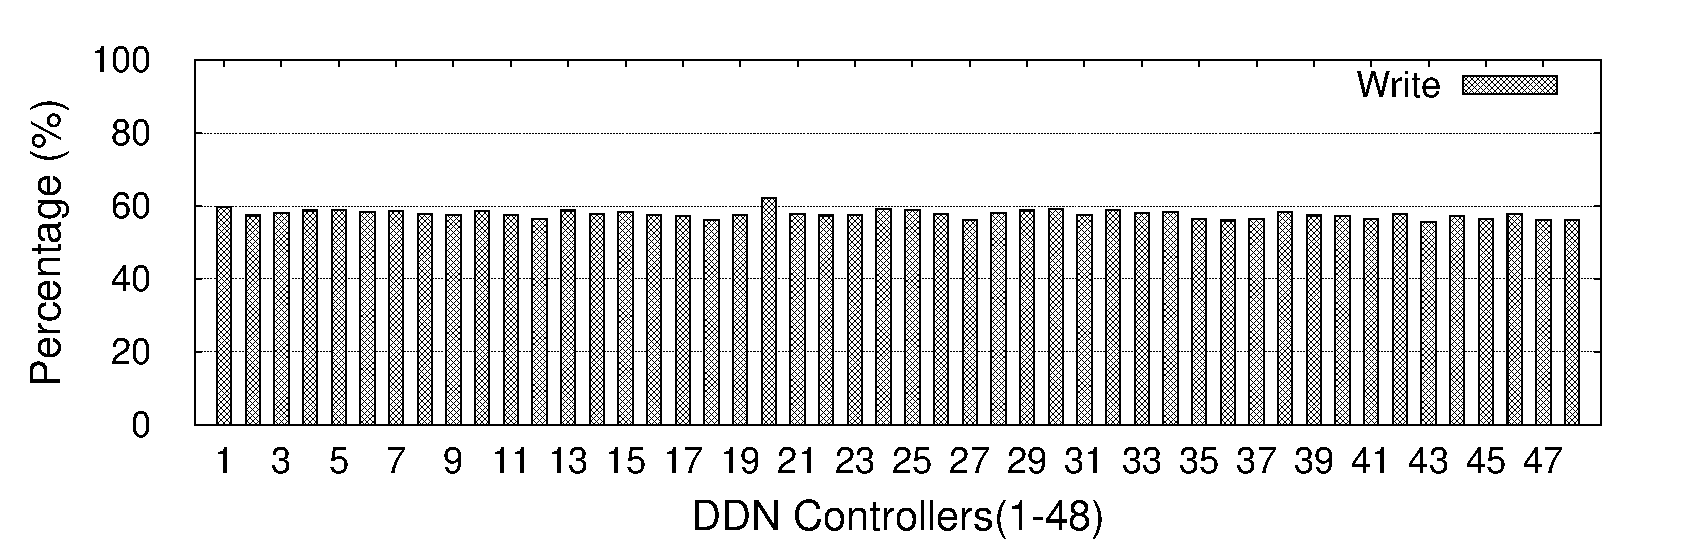
\includegraphics[width=0.5\textwidth]{./figs/spider1-wr-ratio.eps}}\\
{(a) Spider 1}\\
{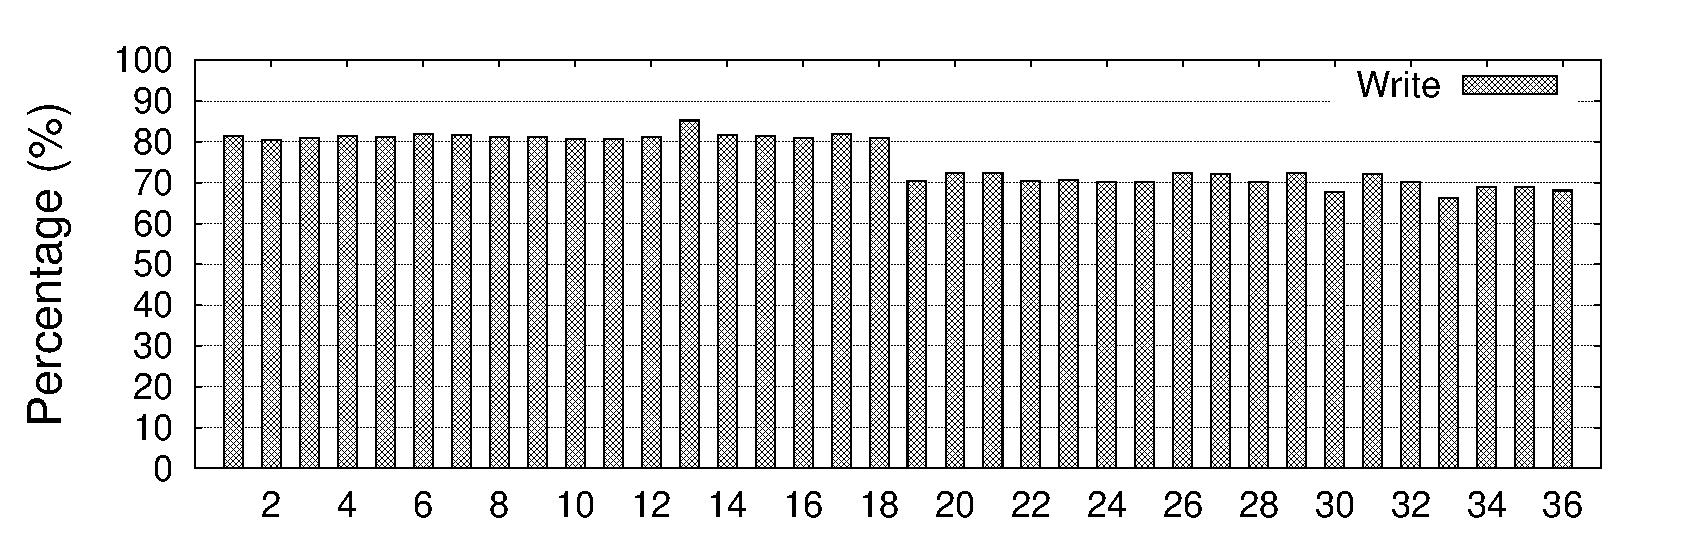
\includegraphics[width=0.5\textwidth]{./figs/spider2-wr-ratio.eps}}\\
{(b) Spider 2}\\
\end{tabular}
\vspace{-0.1in}
\caption{Read vs Write on the Storage System}
\label{fig:rwratio}
\end{center}
\end{figure}

\subsubsection{Peak Bandwidth Usage}

\begin{figure}[!thb]
\begin{center}
\begin{tabular}{c}
{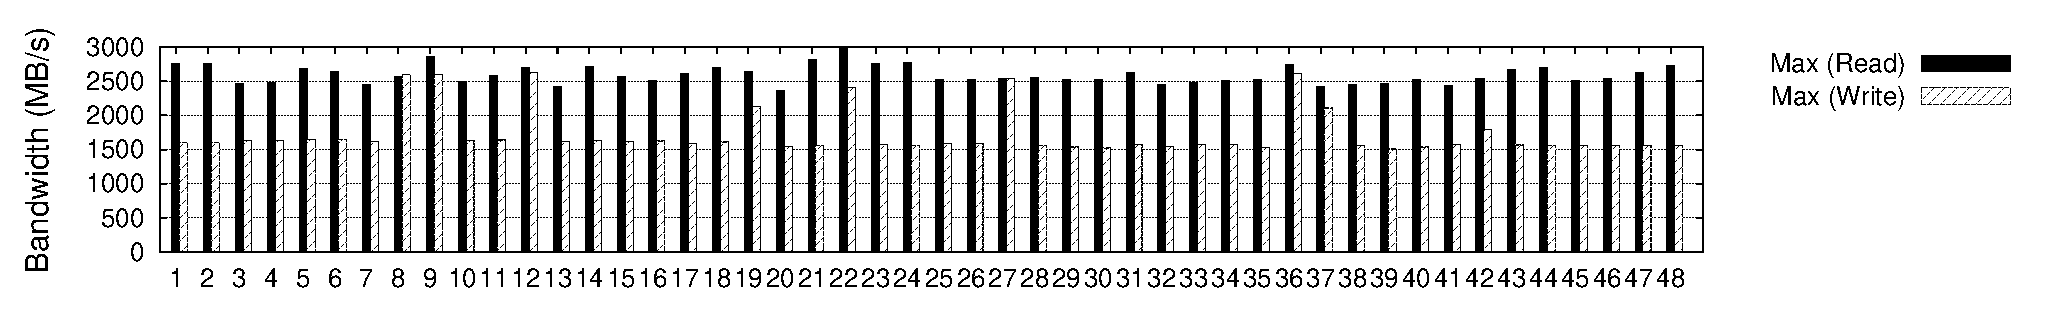
\includegraphics[width=0.50\textwidth]{./figs/spider1-bw-perc-max.eps}}\\
{(a) Spider 1}\\
\\
{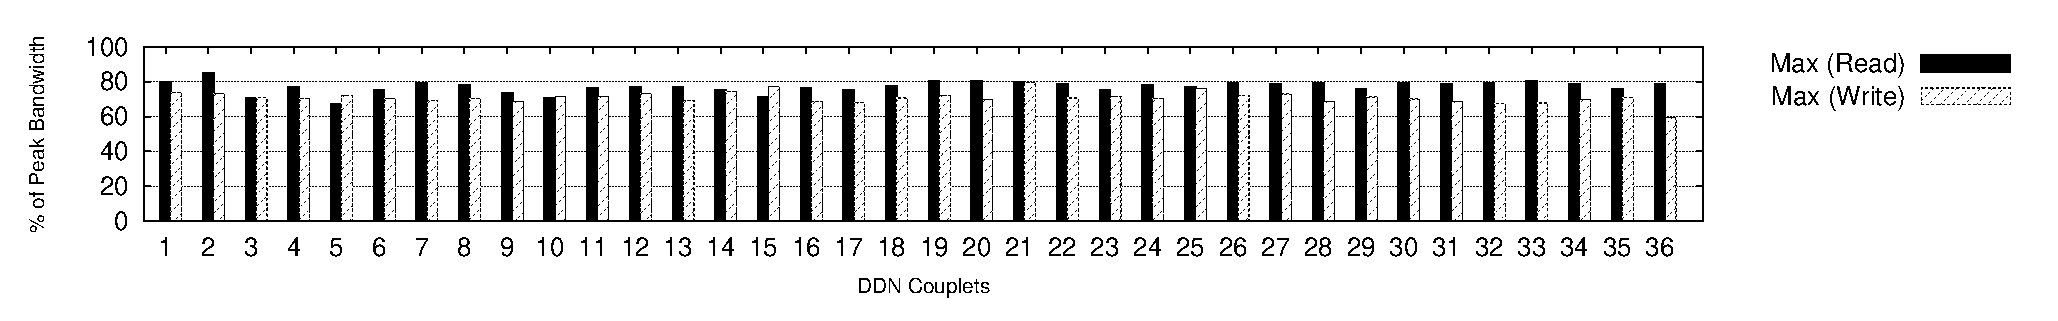
\includegraphics[width=0.50\textwidth]{./figs/spider2-bw-perc-max.eps}}\\
{(b) Spider 2}\\
\end{tabular}
\vspace{-0.1in}
\caption{Peak bandwidth usage at the RAID controllers}
\label{fig:ddnpeakBW}
\end{center}
\end{figure}

\subsubsection{Spider 2 Usage Status}

\begin{figure}[!thb]
\begin{center}
\begin{tabular}{c}
{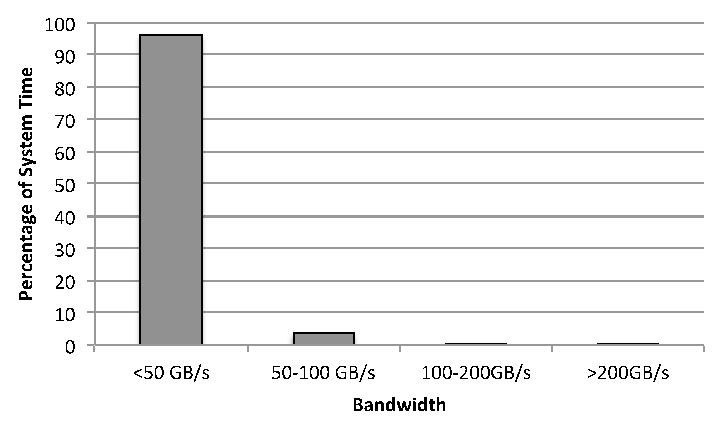
\includegraphics[width=0.40\textwidth]{./figs/bwUsage.eps}}\\
\end{tabular}
\vspace{-0.1in}
\caption{Spider 2 usage with respect to bandwidth}
\label{fig:bwUsage}
\end{center}
\end{figure}



\begin{figure}[!thb]
\begin{center}
\begin{tabular}{c}
{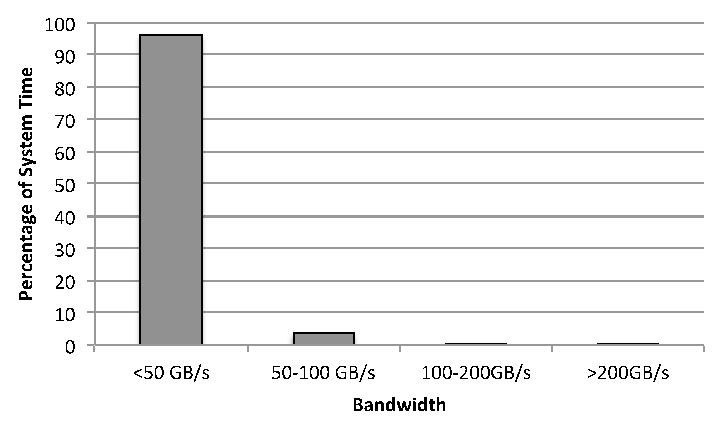
\includegraphics[width=0.40\textwidth]{./figs/storageUsage.eps}}\\
\end{tabular}
\vspace{-0.1in}
\caption{Spider 2 usage with respect to storage space}
\label{fig:storageUsage}
\end{center}
\end{figure}


\subsection{I/O Requests}
\subsubsection{Request Size distribution}



\begin{figure}[!t]
\begin{center}
\begin{tabular}{cc}
\hspace*{-1cm}                                                           
{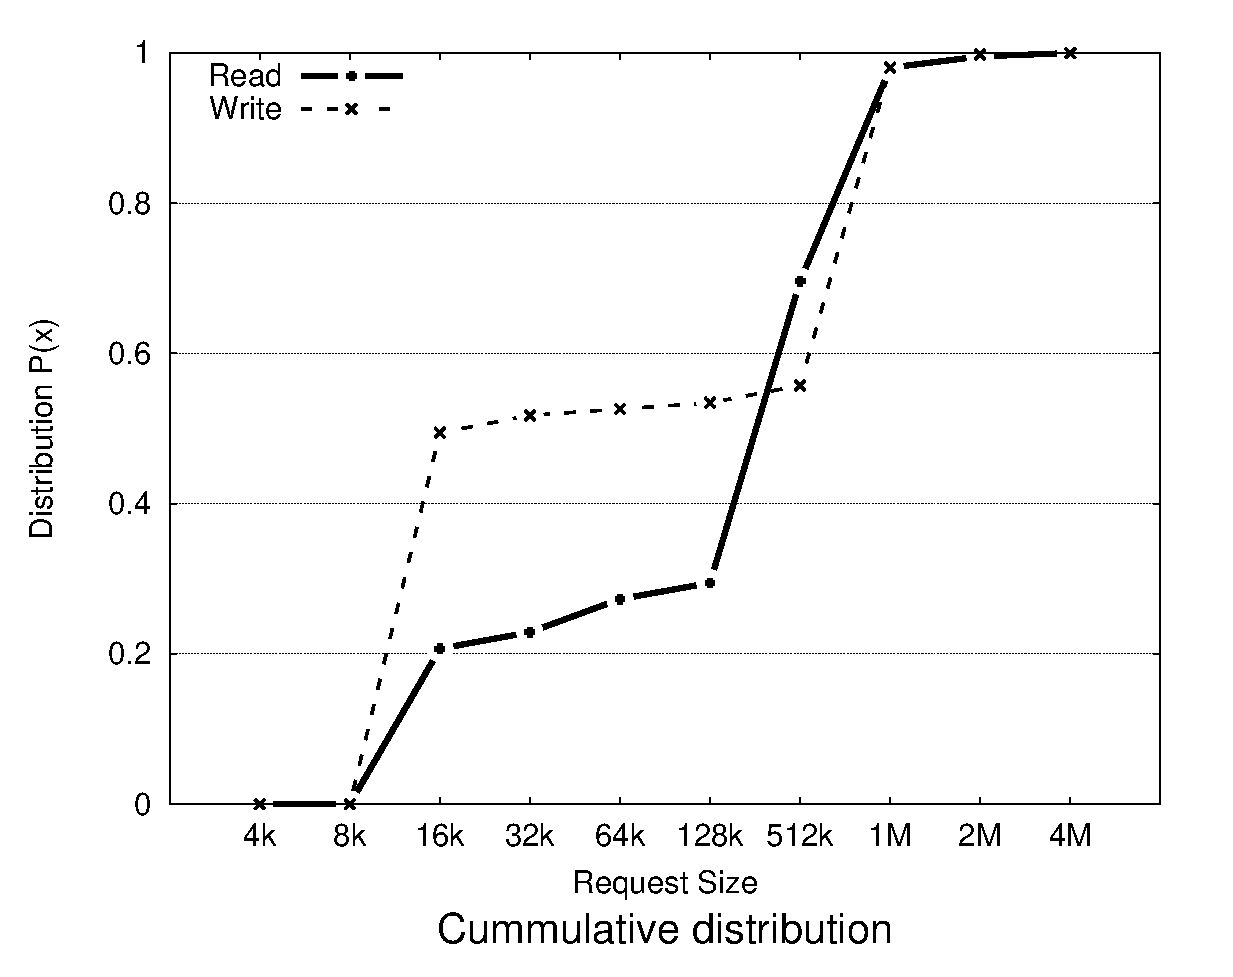
\includegraphics[width=0.27\textwidth]{./figs/spider1-reqSizeCDF.eps}}&
\hspace{-2mm}
{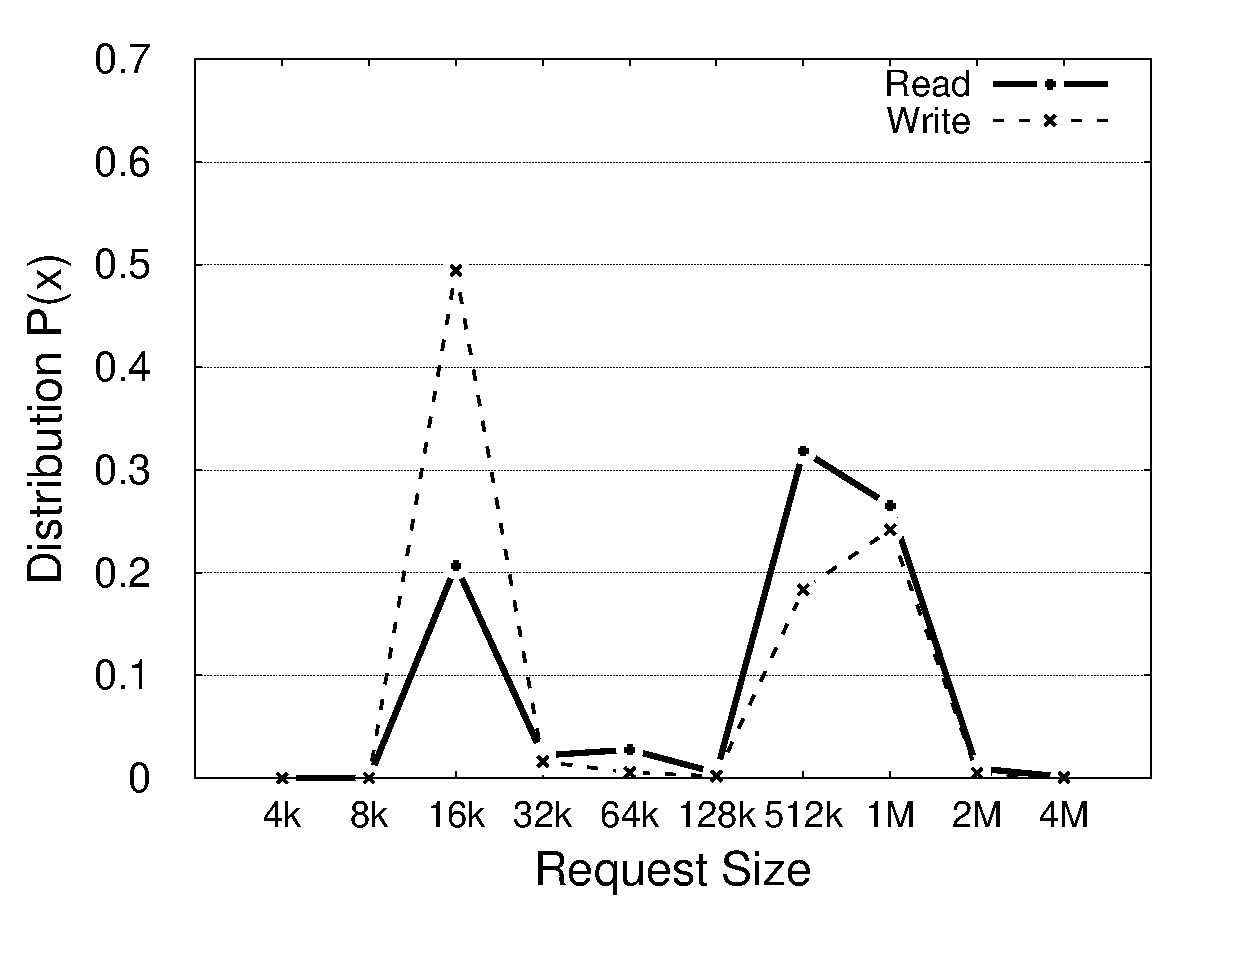
\includegraphics[width=0.27\textwidth]{./figs/spider1-reqSizePDF.eps}}\\
\small (a) CDF & \small(b) PDF \\
\end{tabular}
\vspace{-0.1in}
\captionsetup{justification=centering}
\caption{Spider 1 - Distribution of Request Sizes}
\label{fig:spider1-reqsizedist}
\end{center}
\end{figure}

\begin{figure}[!t]
\begin{center}
\begin{tabular}{cc}
\hspace*{-1cm}                                                           
{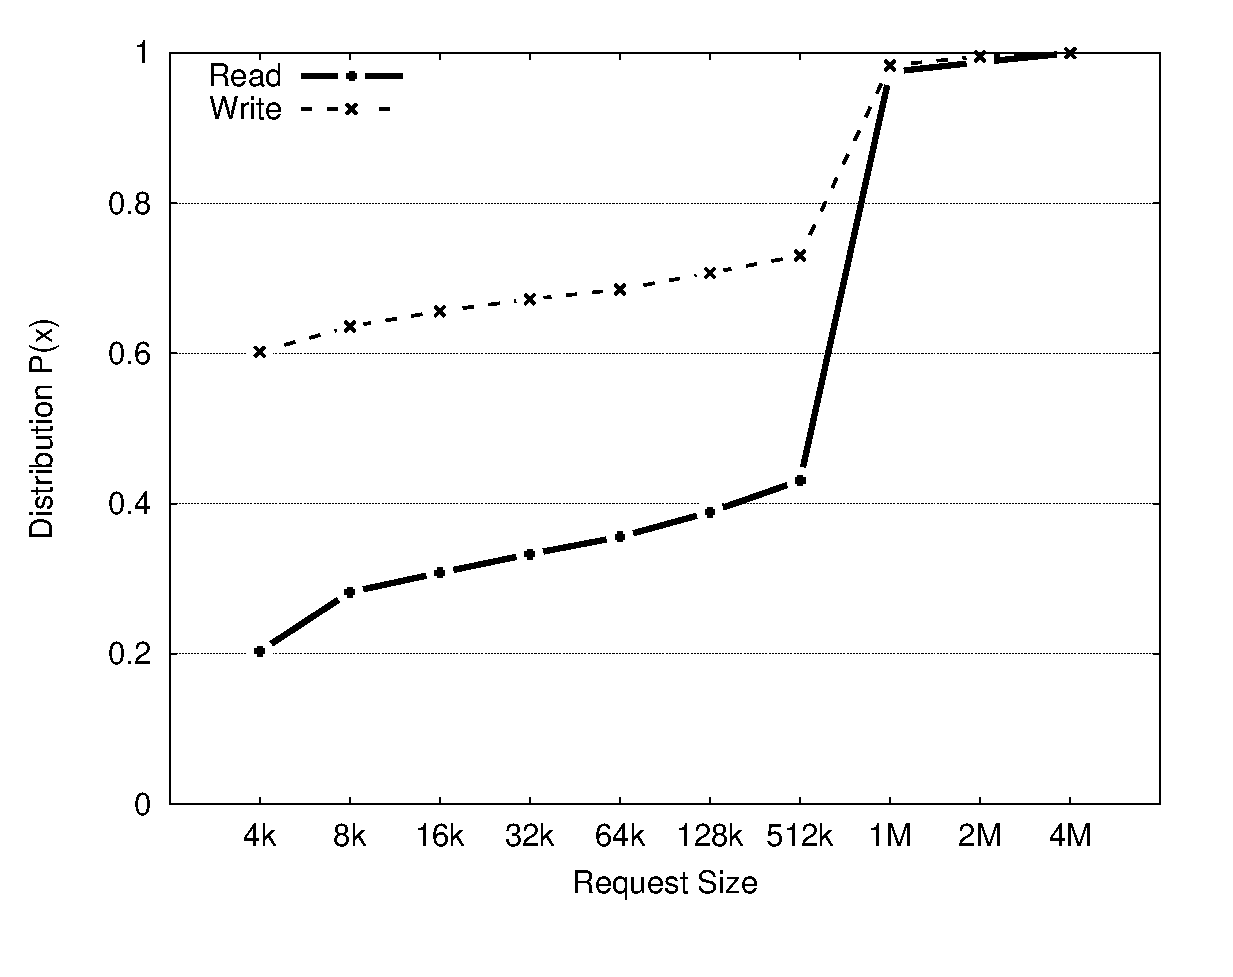
\includegraphics[width=0.27\textwidth]{./figs/spider2-reqSizeCDF.eps}}&
\hspace{-2mm}
{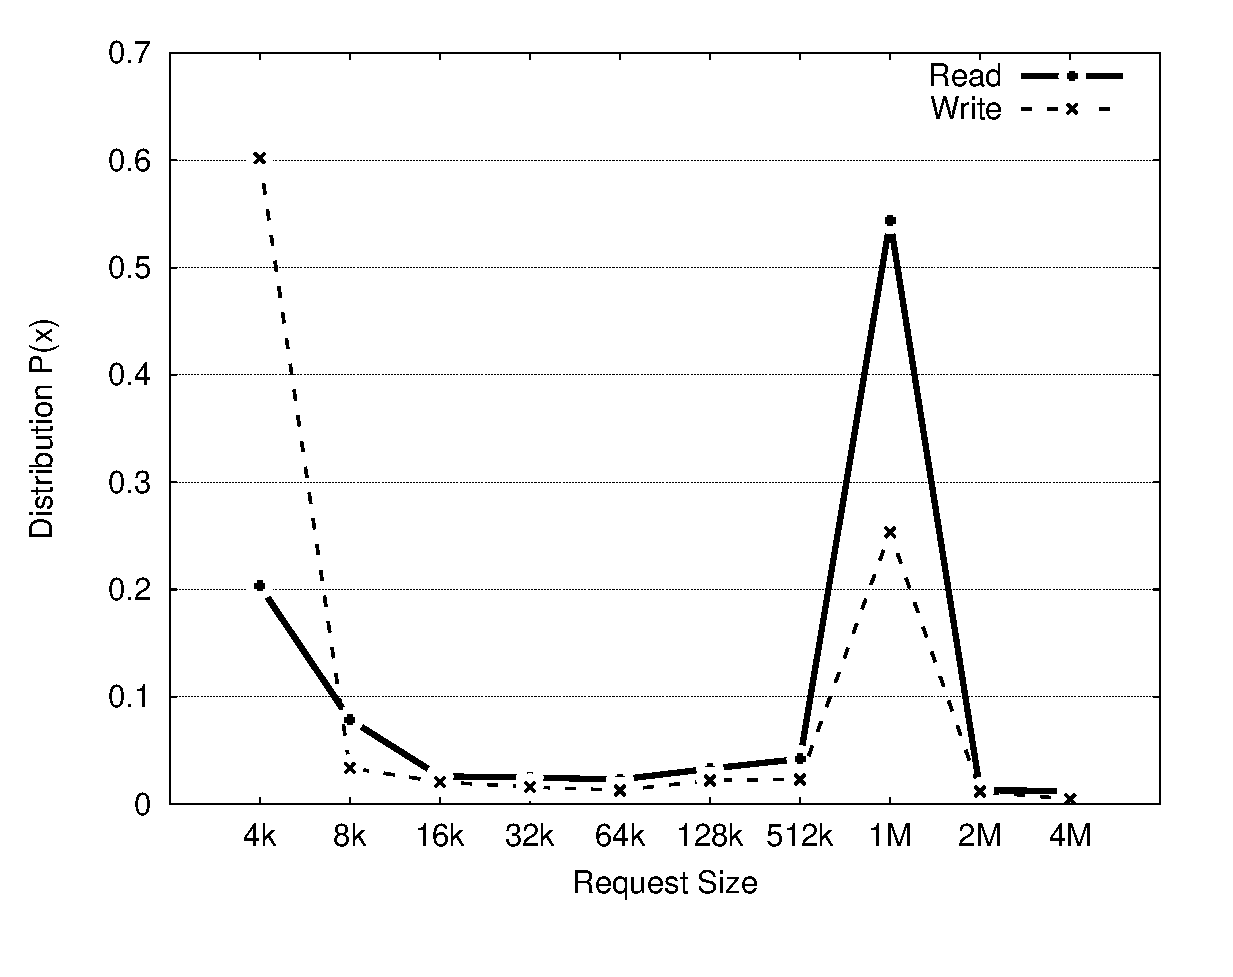
\includegraphics[width=0.27\textwidth]{./figs/spider2-reqSizePDF.eps}}\\
\small (a) CDF & \small(b) PDF \\
\end{tabular}
\vspace{-0.1in}
\caption{Spider 2 - Distribution of Request Sizes}
\label{fig:spider2-reqsizedist}
\end{center}
\end{figure}

Figure~\ref{fig:spider1-reqsizedist} and Figure~\ref{fig:spider2-reqsizedist}
shows the distribution of read and write requests on Spider 1 and Spider 2,
respectively. As can be seen, there are differences. The Lustre file system
supports a range of request block sizes, the smallest being 4 kiloBytes (kB)
and the largest being 4 MegaBytes (MB).  However, on Spider 1, the smallest
block size we were able to monitor was 16KB, a limitation of the DDN RAID
controller. Interpreting from the CDF and PDF plots here are some interesting
observation.

\begin{itemize}

\item  60\% of write requests on Spider 2 are 4kB or less.  In Spider 1, we
unable to distinguish between the 4kB, 8kB and 16kB, which accounted for 50\%
of the write requests. Accounting for this and comparing Spider 1 and 2 file
size distributions, it can be seen that there are 10\% more small block requests (i.e.
smaller than 8kB) on Spider 2, for write operations. Please remember that these
are directly obtained from the DDN controllers not from the file system. One
possible explanation for this increase can be due to the local file system
(ldiskfs) metadata operations. Other possible explanation can be the
controller-level background disk integrity check (i.e. scrubbing) events. Exact
cause of this increase is unknown at this point and it is being investigated.
For read operations, Spider 1 and Spider 2 behave the same for small files, the
distribution has not changed.

\item  For writes, Spider 2 has 70\% of the requests which are less than or
equal to 512kB, whereas on Spider 1, only 55\% of the requests were less than
512kB. It is worth noting that the data presented in this paper are gathered in 
different years, the application versions have changed, and there are a different
mix of applications running as the data were collected. The OLCF traditionally has 
a large mix of applications that have well-formed I/O or are using middleware 
libraries such as ADIOS \cite{adios}. The latest round of applications do not have 
this robustness in their I/O patterns, and have shown to have some pathological 
tendencies; these smaller files and request sizes that are more focused on read 
operations are large performance drains on a system that was designed to perform 
1MB sequential write and read I/O operations. 

\item On Spider 2 over 50\% of reads were 1MB, similar to Spider 1 combined
512kB and 1MB were 50\%. However, only 25\% of writes on Spider 2 are 1MB,
whereas on Spider 1 over 45\% of writes where either 512kB or 1MB. We postulate 
again that the Application workload of the OLCF is different enough at the times of 
measurement to show this difference in the distribution.

\item   On Spider 1, we observed a large number of 512kB requests for both read
and write requests. This was due to problems in the dm-multipath \cite{mpath} 
package that was available for the version of the Linux operating system that was 
employed. This version had a bug that broke up a 1024kB I/O request into 2 
512kB requests. Later versions addressed this performance problem by not breaking 
up the I/O request. Additionally the I/O request scheduler that was used on 
Spider 1 was ``deadline'' which allowed the kernel to re-order some I/O requests. 
In 2011 Spider 1 was moved to the ``noop'' scheduler, and this phenomenon 
disappeared. We see the same drop in 512kB requests for Spider 2 as well. Finally, 
changes to the ib\_srp kernel module allow more queued requests and better memory 
handling of a larger queue through scatter\/gather tables. This allowed fully 
queuing 1024kB requests and pushing them all the way to the DDN controller. As 
a result of these 3 changes the number of 512kB requests have dramatically been 
reduced for Spider 2.
\end{itemize}

\subsubsection{Request Size Latency distribution}

With the new DDN SFA API, now we have the capability of collecting I/O request
service latencies. Figure~\ref{fig:spider1-reqLat} shows Spider 2 request service
latency distributions. Service latency here includes the total sum of the time
spent on the queue and the time spent on fetching/putting data from/to the
disk. As can be seen from the figure, 90\% of reads and more than 80\% write
requests are serviced at most in 16ms and this is the finest granularity the
DDN API can provide. 

The SFA12KX's software incorporates newer caching algorithms that are designed to 
lower the latency for certain operations, and with the readahead cache disabled 
and ReACT\textsuperscript{TM} enabled, we see this highly desirable distribution 
of latencies of 16ms or less.

\begin{itemize}
\item
The SFA12KX disk controller has the ability to analyze incoming I/O request stream
and begin to aggressively read-ahead on the disk to internal cache. The hope is that 
a large read can be sped up by hiding the latency of the seek if the data is in cache.
In our experience and testing, this was a very large hindrance to performance in 
workloads that mimic the many file read operations from Titan's compute nodes. This 
is due to the algorithm caching the wrong data, having to invalidate the cache, 
seek to the location on disk, cache that data, and then repeat with the next read 
request. By disabling the read-ahead cache, we dramatically lower the latency of 
the non-sequential read requests we see in the production environment. 

\item
The Real-time Adaptive Cache Technology (ReACT\textsuperscript{TM})\cite{ReACT} feature was developed
to make the SFA platforms more attractive from an IOPS perspective. The feature's main goal 
is to speed up the performance of the large 1MB write requests, avoiding caching the I/O on the 
partner controller. The decision to only cache <1MB write operations relieves a bottleneck 
that earlier versions of DDN's products did poorly - including the S2A 9900's that 
Spider 1 was constructed of. In earlier versions of the product you could either mirror 
your cache on the partner controller for data resilience in the face of controller 
failure, or you could disable the cache and get performance for the large streaming 1MB 
(or larger) writes. ReACT gives a framework where the best of both worlds can exist. 
A 1MB write can be written directly to disk, which is the lowest latency possible for 
that operation. A 4kB can be written into controller cache and also mirrored to the 
partner controller in about the same amount of time, which is far faster than 
committing that operation to the disk. We feel that this feature has allowed 
Spider 2 to reach the low latencies across the spectrum of write request sizes 
and is a large benefit to our users. 

\end{itemize}


  


\begin{figure}[!t]
\centering
\begin{tabular}{cc}
{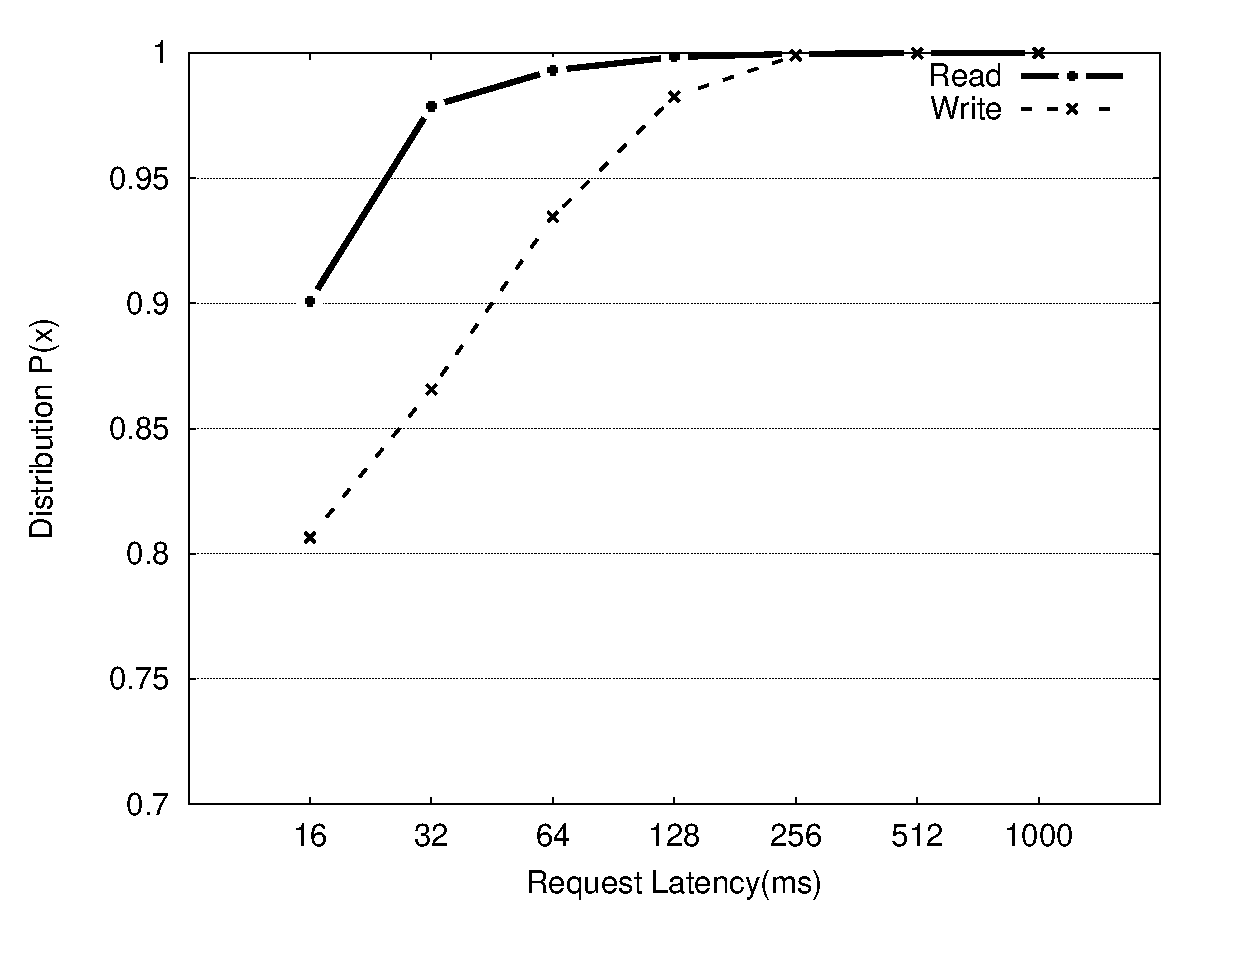
\includegraphics[width=0.24\textwidth]{./figs/spider2-reqLatCDF.eps}}&
{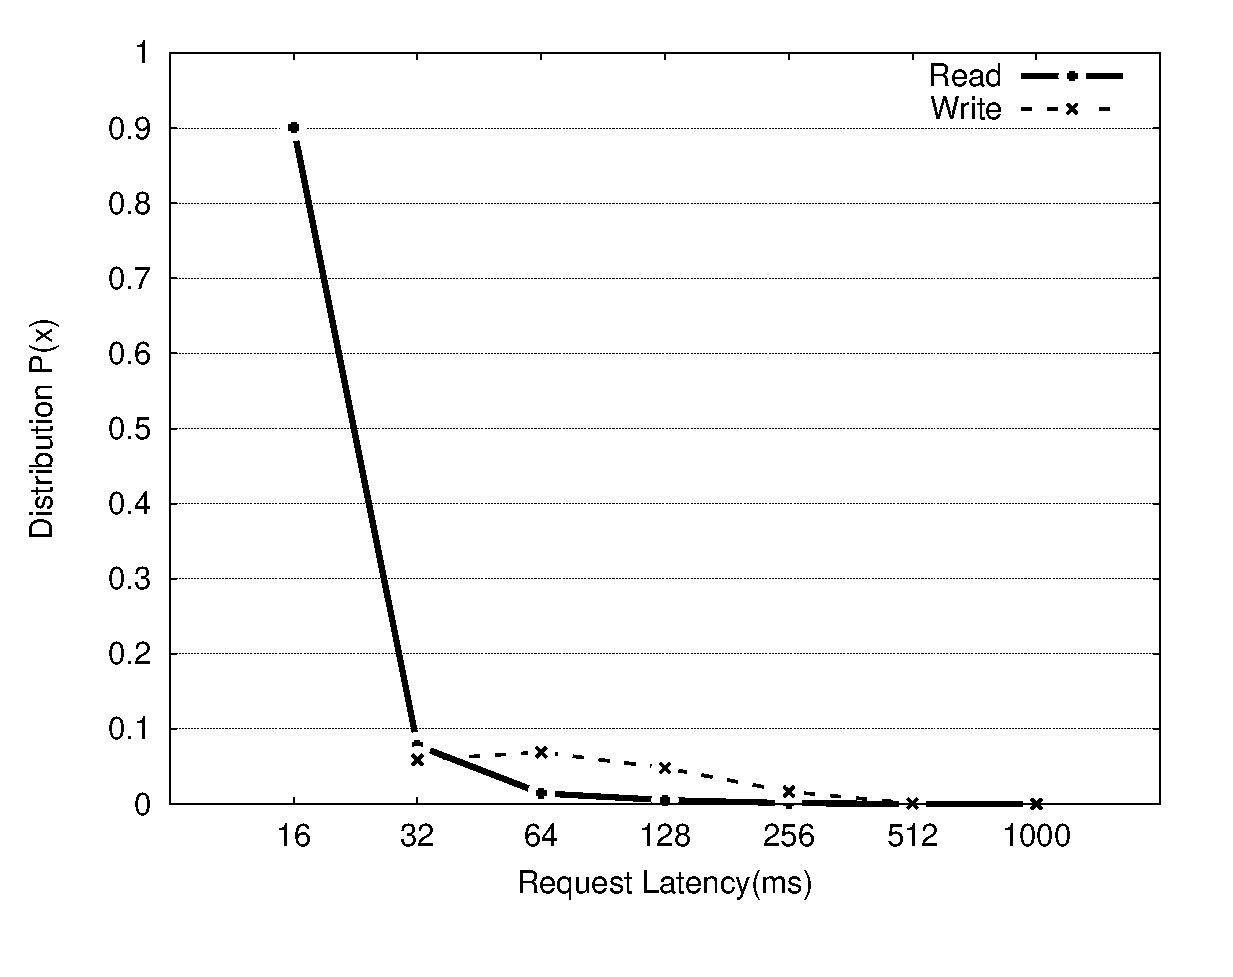
\includegraphics[width=0.24\textwidth]{./figs/spider2-reqLatPDF.eps}}\\
\end{tabular}
\vspace{-0.1in}
\centering
\caption{Spider 2 - Request Service Latency distribution}
\label{fig:spider1-reqLat}
\end{figure}




%\subsection{Request Size vs Bandwidth}

 
